%%%%%%%%%%%%%%%%%%%%%%%%%%%%%%%%%%%%%%%%%%%%%%%%%%%%%%%%%%%%%%%%%%%%%%%%%%%%%%%%%%
\begin{frame}[fragile]\frametitle{}
\begin{center}
{\Large How LLMs work?}

{\tiny (Ref: What Is ChatGPT Doing \ldots and Why Does It Work? - Stephan Wolfram)}

\end{center}
\end{frame}


%%%%%%%%%%%%%%%%%%%%%%%%%%%%%%%%%%%%%%%%%%%%%%%%%%%%%%%%%%%
\begin{frame}[fragile]\frametitle{What is Language Model}

\begin{itemize}
\item what ChatGPT is always fundamentally trying to do is to produce a ''reasonable continuation'' of whatever text it's got so far
\item Language model : predicting the next word
\item SO, for the text ``The best thing about AI is its ability to'', what could be the next best word?
\item  it doesn’t look at literal text; it looks for things that in a certain sense ''match in meaning''. But the end result is that it produces a ranked list of words that might follow, together with ''probabilities'':
\item And doing this over and over again ''given the text so far, what should the next word be?''—and each time adding a word.
\end{itemize}	

\begin{center}
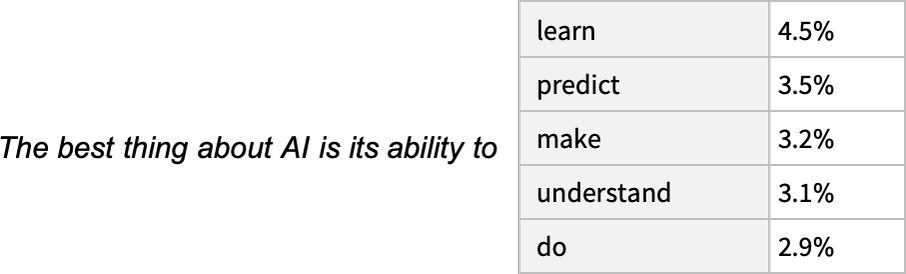
\includegraphics[width=0.6\linewidth,keepaspectratio]{llm1}
\end{center}

\end{frame}

%%%%%%%%%%%%%%%%%%%%%%%%%%%%%%%%%%%%%%%%%%%%%%%%%%%%%%%%%%%
\begin{frame}[fragile]\frametitle{Best or lesser than Best?}

\begin{itemize}
\item  ''highest-ranked'' word (i.e. highest ''probability'') seems correct, right?
\item  Ok for more deterministic, scientific writings (a very ''flat'' essay) but for more fluid, creative writing less than perfect is actually better.
\item  ''temperature'' parameter that determines how often lower-ranked words will be used, 0.8 seems best
\end{itemize}	


\end{frame}


%%%%%%%%%%%%%%%%%%%%%%%%%%%%%%%%%%%%%%%%%%%%%%%%%%%%%%%%%%%
\begin{frame}[fragile]\frametitle{Probability of the next word}

\begin{itemize}
\item Simple idea would be, for the current word, find the 'most occurring' next word from the training corpus, ie whole internet or all books or can be small as past SMS in your mobile.
\item So, that's basically a huge search and aggregations to compute probabilities for all the words in the rest of the vocabulary.
\end{itemize}	

\begin{center}
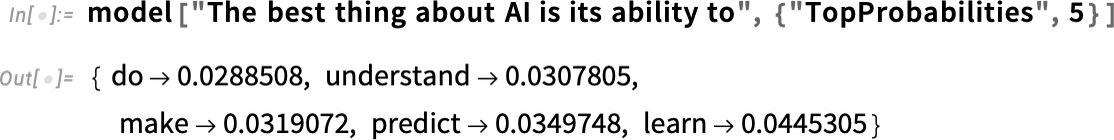
\includegraphics[width=0.8\linewidth,keepaspectratio]{llm2}

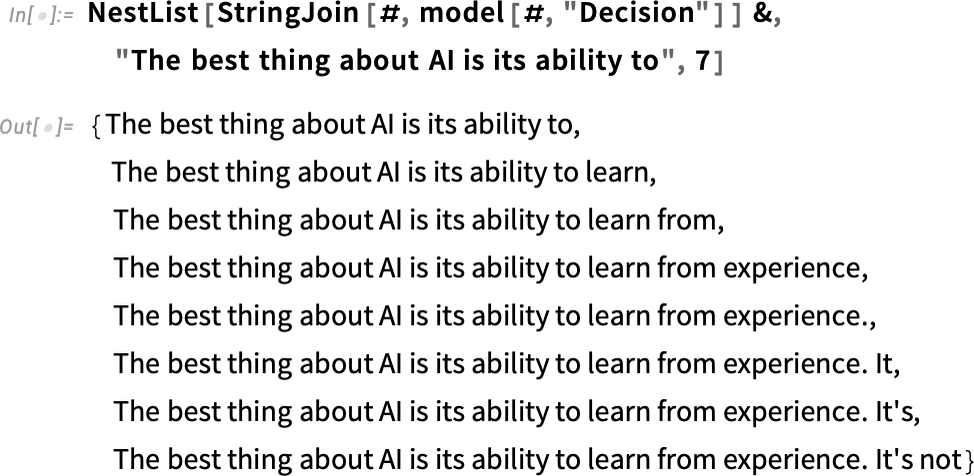
\includegraphics[width=0.6\linewidth,keepaspectratio]{llm3}
\end{center}


\end{frame}

%%%%%%%%%%%%%%%%%%%%%%%%%%%%%%%%%%%%%%%%%%%%%%%%%%%%%%%%%%%
\begin{frame}[fragile]\frametitle{Problem}

What happens if one goes on longer? In this (''zero temperature'') case what comes out soon gets rather confused and repetitive:

\begin{center}
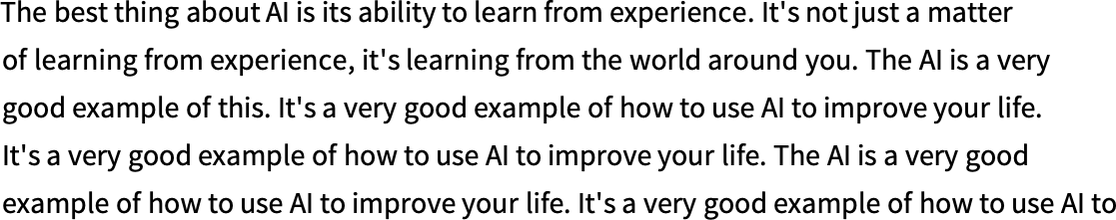
\includegraphics[width=0.8\linewidth,keepaspectratio]{llm4}
\end{center}

with the ''randomness'' corresponding to ''temperature'' 0.8? And every time one does this, different random choices will be made, and the text will be different—as in these 5 examples:

\begin{center}
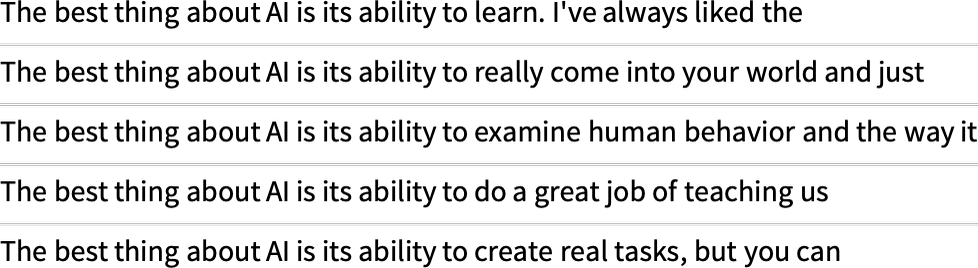
\includegraphics[width=0.6\linewidth,keepaspectratio]{llm5}
\end{center}

So what happens if one goes on longer? Here’s a random example. It’s better than the top-word (zero temperature) case, but still at best a bit weird

\end{frame}


%%%%%%%%%%%%%%%%%%%%%%%%%%%%%%%%%%%%%%%%%%%%%%%%%%%%%%%%%%%
\begin{frame}[fragile]\frametitle{A simpler example}

\begin{itemize}
\item  Instead of predicting the next word, predict the next characters.
\item So 26 chars. Plus space punctuation, numbers, etc, say 50 options.
\item so given the current char, whats the next best char?
\end{itemize}	

\begin{center}
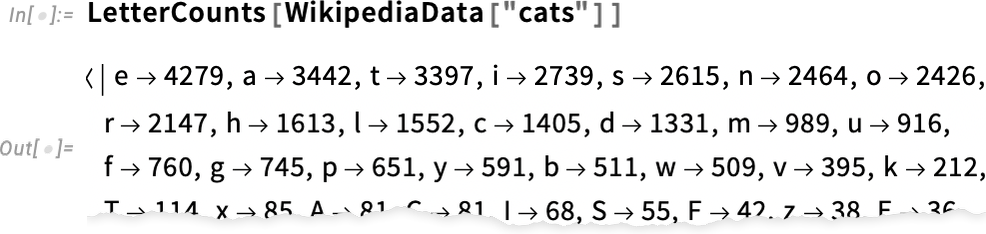
\includegraphics[width=0.8\linewidth,keepaspectratio]{llm6}

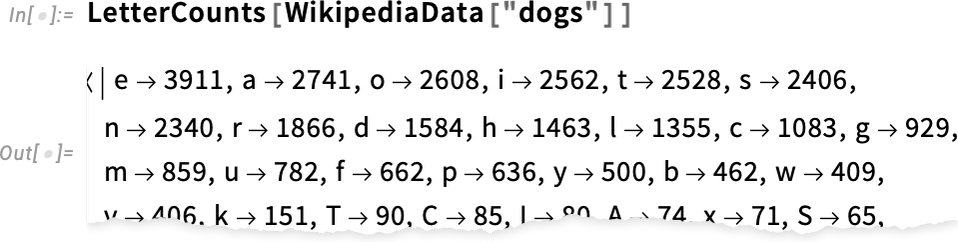
\includegraphics[width=0.8\linewidth,keepaspectratio]{llm7}

\end{center}

The results are similar, but not the same (''o'' is no doubt more common in the ''dogs'' article because, after all, it occurs in the word ''dog'' itself)
\end{frame}

%%%%%%%%%%%%%%%%%%%%%%%%%%%%%%%%%%%%%%%%%%%%%%%%%%%%%%%%%%%
\begin{frame}[fragile]\frametitle{The problem}

Here’s a sample of what we get if we just generate a sequence of letters with these probabilities:

\begin{center}
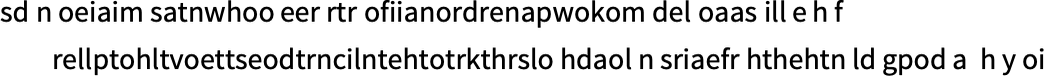
\includegraphics[width=\linewidth,keepaspectratio]{llm8}
\end{center}

We didn’t happen to get any ''actual words'' here. Lets try two chars at a time, ie bi-grams. For 'q' having 'u' next has highest probability.

\begin{center}
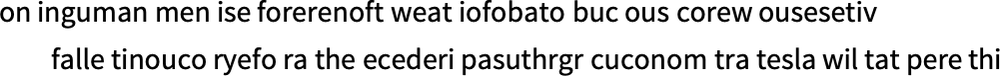
\includegraphics[width=\linewidth,keepaspectratio]{llm9}
\end{center}

\end{frame}

%%%%%%%%%%%%%%%%%%%%%%%%%%%%%%%%%%%%%%%%%%%%%%%%%%%%%%%%%%%
\begin{frame}[fragile]\frametitle{Back to words}

\begin{itemize}
\item There are about 40,000 reasonably commonly used words in English.
\item generating ''sentences'', in which each word is independently picked at random, with the same probability that it appears in the corpus. 

\begin{center}
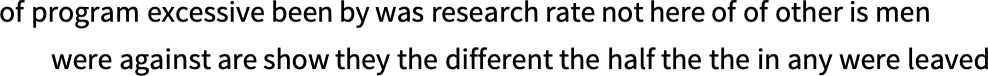
\includegraphics[width=\linewidth,keepaspectratio]{llm10}
\end{center}

\item Not surprisingly, this is nonsense.
\item by giving some seed 'cat'

\begin{center}
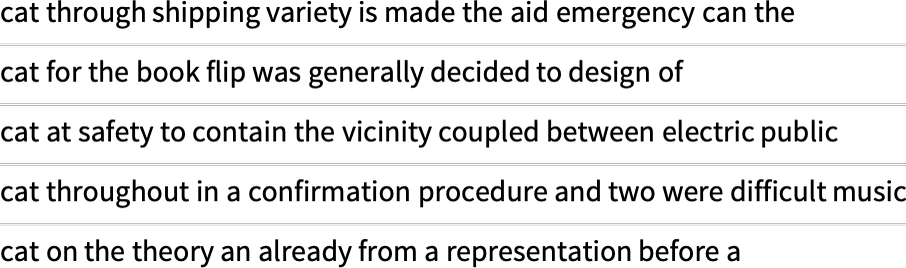
\includegraphics[width=0.8\linewidth,keepaspectratio]{llm11}
\end{center}

\end{itemize}

\end{frame}

%%%%%%%%%%%%%%%%%%%%%%%%%%%%%%%%%%%%%%%%%%%%%%%%%%%%%%%%%%%
\begin{frame}[fragile]\frametitle{n-grams}

\begin{itemize}

\item Similarly, instead using only the current word for predicting the next word, can we use bi-grams, ie 2 words. 
\item Search for this pair in corpus and then find the next best word.
\item But with 40,000 common words, even the number of possible 2-grams is already 1.6 billion—and the number of possible 3-grams is 60 trillion.
\item Combinatorial explosion and search nightmare
\end{itemize}


Whats the solution? Answer: A model 

ChatGPT is precisely a so-called ''large language model'' (LLM) that’s been built to do a good job of estimating those probabilities

\end{frame}

%%%%%%%%%%%%%%%%%%%%%%%%%%%%%%%%%%%%%%%%%%%%%%%%%%%%%%%%%%%
\begin{frame}[fragile]\frametitle{What Is a Model?}

\begin{itemize}
\item Instead of storing all the data points, can we find a governing relation or equation?
\item Let’s imagine we have (somewhat idealized) data for how long the cannon ball takes to fall from various floors:

\begin{center}
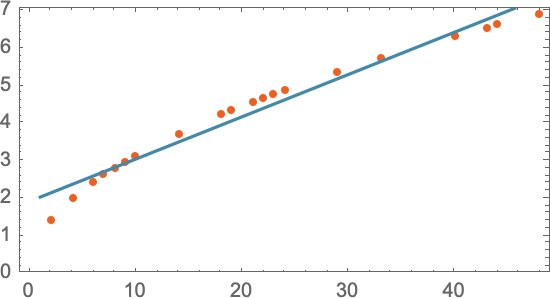
\includegraphics[width=\linewidth,keepaspectratio]{llm12}
\end{center}

\item Approximate but simple, needs only 2 parameters to represent (slope and intercept)

\end{itemize}

\end{frame}

%%%%%%%%%%%%%%%%%%%%%%%%%%%%%%%%%%%%%%%%%%%%%%%%%%%%%%%%%%%
\begin{frame}[fragile]\frametitle{What Is a Model?}

\begin{itemize}
\item Any model you use has some particular underlying structure—then a certain set of ''knobs you can turn'' (i.e. parameters you can set) to fit your data. And in the case of ChatGPT, lots of such ''knobs'' are used—actually, 175 billion of them.
\item Parameters have be adjusted by huge self-supervised, supervised and reinforcement based training.
\item with ''just'' 175B  parameters it is sufficient to make a model that computes next-word probabilities ''well enough'' to give us reasonable essay-length pieces of text.
\end{itemize}

\end{frame}

%%%%%%%%%%%%%%%%%%%%%%%%%%%%%%%%%%%%%%%%%%%%%%%%%%%%%%%%%%%
\begin{frame}[fragile]\frametitle{Generative vs Discriminative}
\begin{columns}
    \begin{column}[T]{0.6\linewidth}
Discriminative Models:
\begin{itemize}
    \item Learn decision boundaries that separate different classes.
    \item Maximize the conditional probability: $P(Y|X)$ — Given $X$, maximize the probability of label $Y$.
    \item Specifically meant for classification tasks.
\end{itemize}

Generative Models
\begin{itemize}
    \item Maximize the joint probability: $P(X, Y)$.
    \item Learn the class-conditional distribution $P(X|Y)$.
    \item Typically not preferred for solving downstream classification tasks.
\end{itemize}
    \end{column}
    \begin{column}[T]{0.4\linewidth}
		\begin{center}
		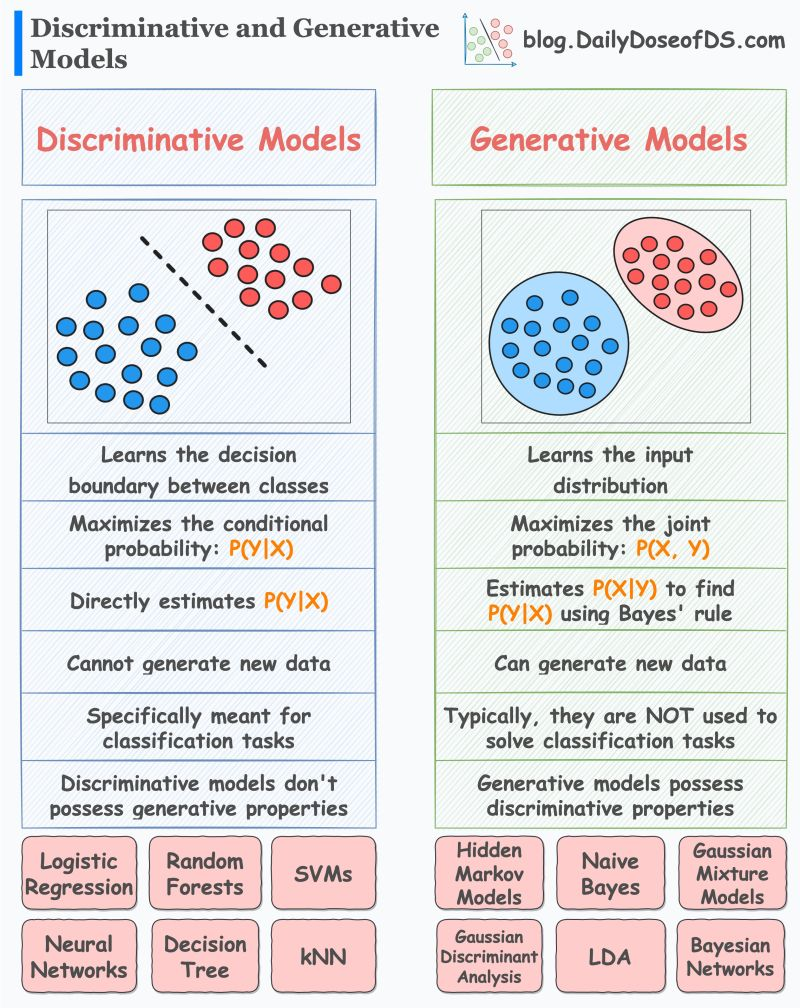
\includegraphics[width=0.6\linewidth,keepaspectratio]{llm64}
		\end{center}
		
		{\tiny (Ref: LinkedIn post on Machine Learning Community by Avi Chawla on 11 Aug 2023 )}
    \end{column}
  \end{columns}
\end{frame}

%%%%%%%%%%%%%%%%%%%%%%%%%%%%%%%%%%%%%%%%%%%%%%%%%%%%%%%%%%%
\begin{frame}[fragile]\frametitle{Generative Models' Capabilities}

\begin{itemize}
    \item Learn the underlying distribution.
    \item Can generate new samples. Discriminative models cannot generate new samples.
	\item Generative models possess discriminative properties: Can be used for classification tasks (if needed).
\end{itemize}

\end{frame}

%%%%%%%%%%%%%%%%%%%%%%%%%%%%%%%%%%%%%%%%%%%%%%%%%%%%%%%%%%%
\begin{frame}[fragile]\frametitle{Word Embedding}

\begin{itemize}
\item ChatGPT is based on Transformer architecture.
\item Encoder part does word embedding, meaning, it captures atleast contextual meaning ie similarity.

\begin{center}
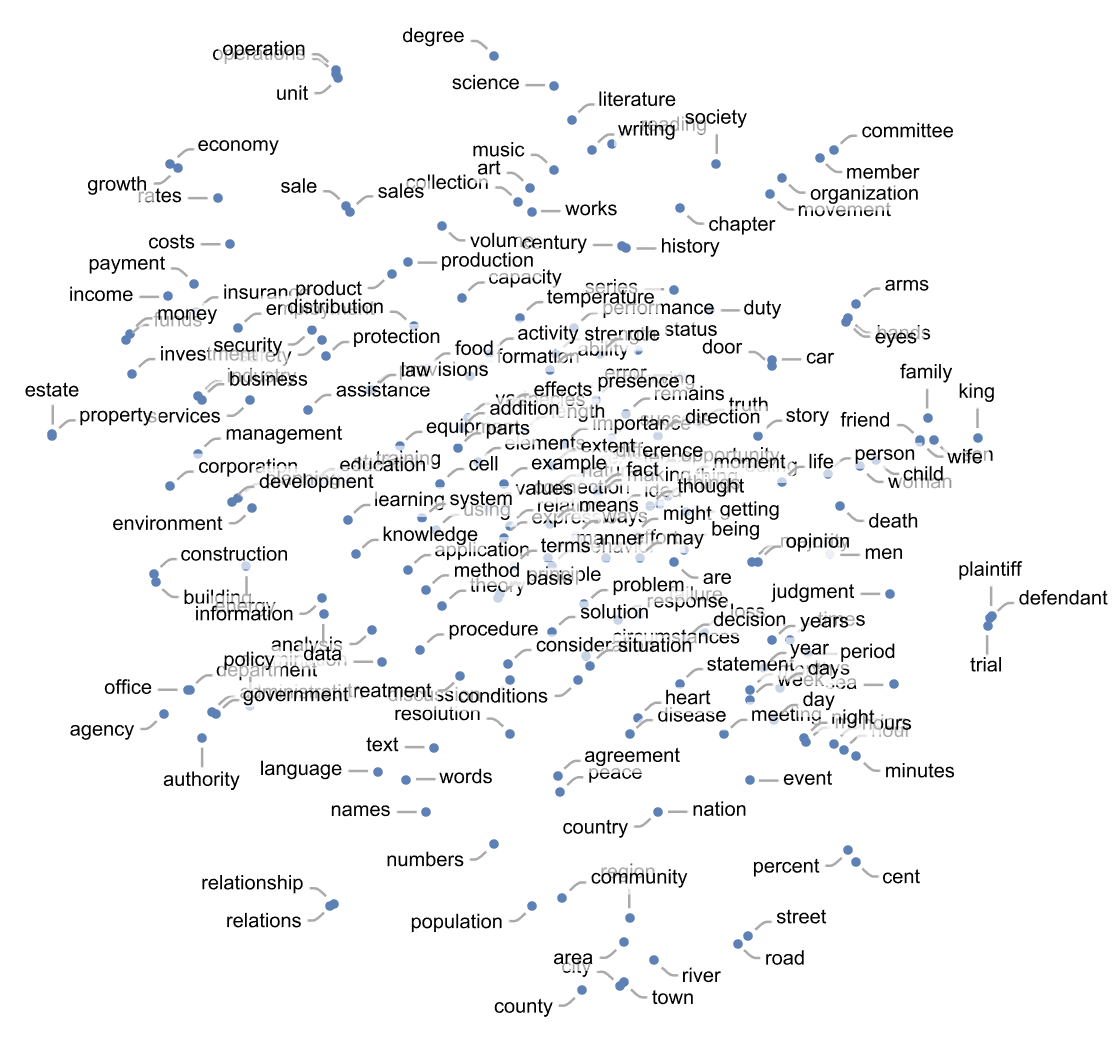
\includegraphics[width=0.6\linewidth,keepaspectratio]{llm13}
\end{center}

\end{itemize}

\end{frame}


%%%%%%%%%%%%%%%%%%%%%%%%%%%%%%%%%%%%%%%%%%%%%%%%%%%%%%%%%%%
\begin{frame}[fragile]\frametitle{Word Embedding}

\begin{itemize}

\item here’s how words corresponding to different parts of speech get laid out:

\begin{center}
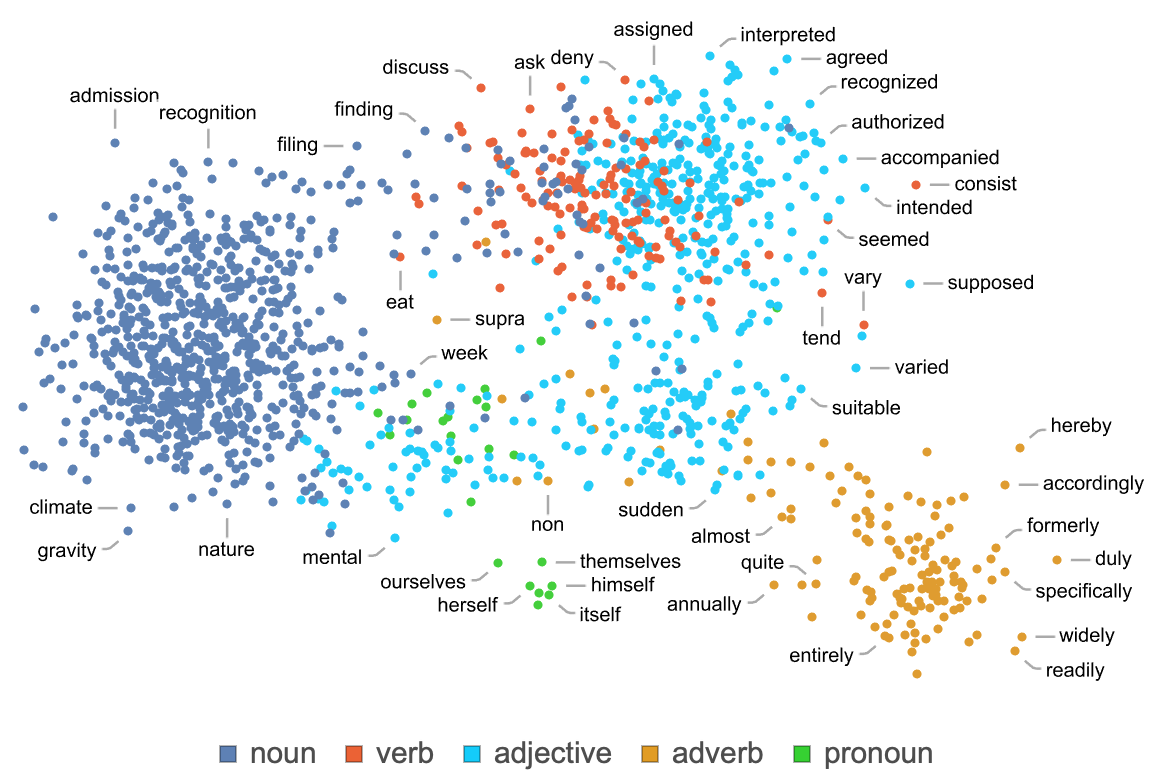
\includegraphics[width=0.6\linewidth,keepaspectratio]{llm14}
\end{center}

\end{itemize}

\end{frame}



%%%%%%%%%%%%%%%%%%%%%%%%%%%%%%%%%%%%%%%%%%%%%%%%%%%%%%%%%%%
\begin{frame}[fragile]\frametitle{Word Embedding}

\begin{itemize}

\item A single word ``crane'' in different sentence context can be 

\begin{center}
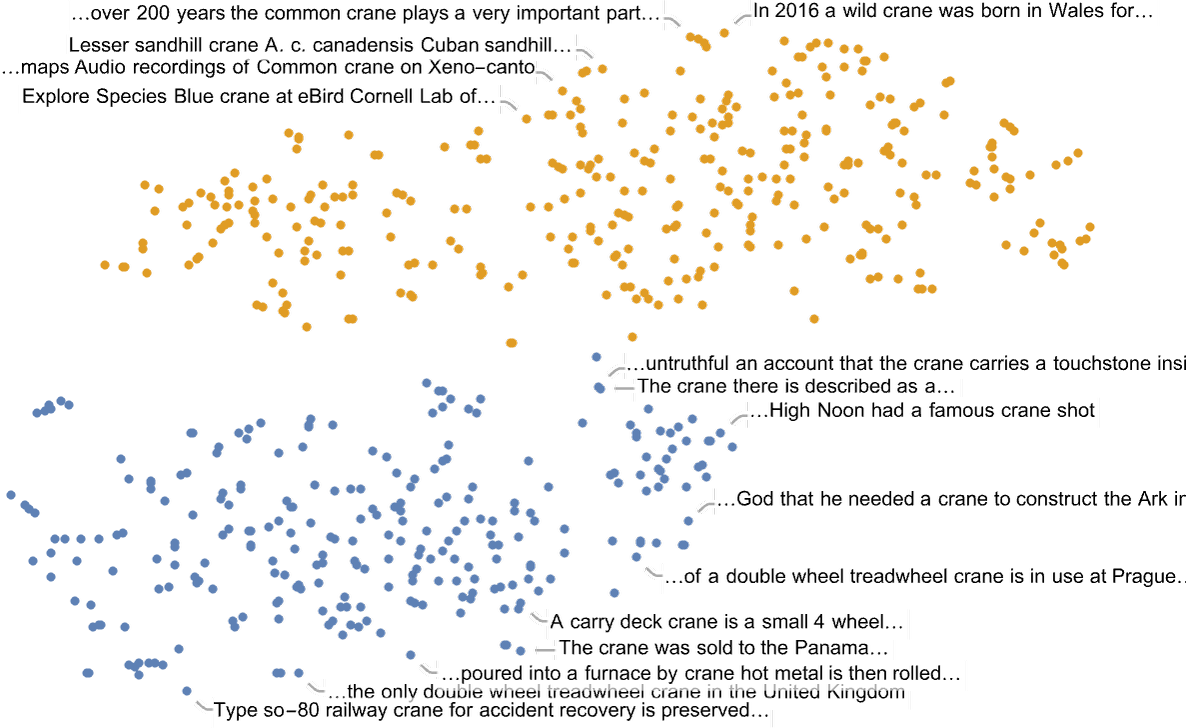
\includegraphics[width=0.6\linewidth,keepaspectratio]{llm15}
\end{center}

\item Thus, even if actual words could be different, but if their semantically similar then ChatGPT response is also similar.
\end{itemize}

\end{frame}

%%%%%%%%%%%%%%%%%%%%%%%%%%%%%%%%%%%%%%%%%%%%%%%%%%%%%%%%%%%
\begin{frame}[fragile]\frametitle{Embeddings}


\begin{itemize}
\item Embeddings capture the semantic meaning of words using dense, low-dimensional vectors.
\item They are trained using neural network models like BERT, Word2Vec, GloVe, or FastText on large corpora.
\item Embeddings can be contextualized or non-contextualized.
\item Contextualized embeddings depend on the surrounding tokens, allowing polysemous words to have unique embeddings.
\item Non-contextualized embeddings are static and pre-trained, such as Word2Vec, GloVe, and FastText.
\item To obtain a token's embedding, extract the learned weights from the trained model for that word.
\item These weights form dense vectors that represent the word's embedding.
\end{itemize}

				
{\tiny (Ref: Overview of Large Language Models - Aman AI)}

\end{frame}


%%%%%%%%%%%%%%%%%%%%%%%%%%%%%%%%%%%%%%%%%%%%%%%%%%%%%%%%%%%
\begin{frame}[fragile]\frametitle{What Is ChatGPT Doing, and Why Does It Work?}

\begin{itemize}
\item ChatGPT is “merely” pulling out some “coherent thread of text” from the “statistics of conventional wisdom” that it’s accumulated. But it’s amazing how human-like the results are.
\item that human language (and the patterns of thinking behind it) are somehow simpler and more “law like” in their structure than we thought. ChatGPT has implicitly discovered it.
\end{itemize}

\end{frame}

%%%%%%%%%%%%%%%%%%%%%%%%%%%%%%%%%%%%%%%%%%%%%%%%%%%%%%%%%%%
\begin{frame}[fragile]\frametitle{Decoder Inference}

\begin{itemize}
\item Decoder models like GPT work by taking a prompt as input and generating text that is consistent with the prompt. 
\item The input prompt is typically a sequence of tokens, which are then fed into the decoder model. 
\item The decoder model then generates the output sequence by attending to the input sequence through self-attention mechanisms.
\item The self-attention mechanisms allow the decoder model to learn the relationships between the tokens in the input sequence. This allows the decoder model to generate output that is consistent with the prompt, even if the prompt is incomplete or ambiguous.
\end{itemize}

\end{frame}

%%%%%%%%%%%%%%%%%%%%%%%%%%%%%%%%%%%%%%%%%%%%%%%%%%%%%%%%%%%
\begin{frame}[fragile]\frametitle{Decoder Inference}

The completion process typically works as follows:

\begin{itemize}
\item The decoder model is given the prompt as input.
\item The decoder model attends to the input sequence through self-attention mechanisms.
\item The decoder model generates the first token in the output sequence.
\item The decoder model attends to the output sequence so far, as well as the input sequence, through self-attention mechanisms.
\item The decoder model generates the next token in the output sequence.
\item Steps 4 and 5 are repeated until the desired length of the output sequence is reached.
\end{itemize}

\end{frame}

%%%%%%%%%%%%%%%%%%%%%%%%%%%%%%%%%%%%%%%%%%%%%%%%%%%%%%%%%%%
\begin{frame}[fragile]\frametitle{In nutshell}

ChatGPT works like:
\begin{itemize}
\item Ingest an enormous corpus of text and while so doing, assign to each unique word a unique identifier, a number that will serve as a token to represent that word, record the location of every token relative to every other token.
\item Leveraging this map, given any string of words as a prompt, use the neural network to predict the next word (just like AutoCorrect).
\item Based on feedback from so doing, adjust the internal parameters of the neural network to improve its performance.
\item As performance improves, extend the reach of prediction from the next word to the next phrase, then to the next clause, the next sentence, the next paragraph, and so on, improving performance at each stage by using feedback to further adjust its internal parameters.
\item Based on all of the above, generate text responses to user questions and prompts that reviewers agree are appropriate and useful.
\end{itemize}


{\tiny (Ref: Understanding ChatGPT: A Triumph of Rhetoric - Geoffrey Moore)}

\end{frame}

%%%%%%%%%%%%%%%%%%%%%%%%%%%%%%%%%%%%%%%%%%%%%%%%%%%%%%%%%%%
\begin{frame}[fragile]\frametitle{Bottom-line}

\begin{itemize}
\item ChatGPT has no ideas of any kind—no knowledge or expertise—because it has no semantic information. 
\item It is all math. Math has been used to strip words of their meaning, and that meaning is not restored until a reader or user engages with the output to do so, using their own brain, not ChatGPT’s. 
\item ChatGPT is operating entirely on form and not an iota on content. 
\item By processing the entirety of its corpus, it can generate the most probable sequence of words that correlates with the input prompt it had been fed. 
\item Additionally, it can modify that sequence based on subsequent interactions with an end user. 
\item As human beings participating in that interaction, we process these interactions as a natural language conversation with an intelligent agent, but that is not what is happening at all. 
\item ChatGPT is using our prompts to initiate a mathematical exercise using tokens and locations as its sole variables. 
\end{itemize}


{\tiny (Ref: Understanding ChatGPT: A Triumph of Rhetoric - Geoffrey Moore)}

\end{frame}

%%%%%%%%%%%%%%%%%%%%%%%%%%%%%%%%%%%%%%%%%%%%%%%%%%%%%%%%%%%%%%%%%%%%%%%%%%%%%%%%%%
\begin{frame}[fragile]\frametitle{}
\begin{center}
{\Large Reinforcement Learning from Human Feedback (RLHF)}

{\tiny (Ref: Linkedin Post on 11 Aug 2023 by -Katharina Koerner)}

\end{center}
\end{frame}

%%%%%%%%%%%%%%%%%%%%%%%%%%%%%%%%%%%%%%%%%%%%%%%%%%%%%%%%%%%
\begin{frame}[fragile]\frametitle{What is RLHF?}

\begin{itemize}
\item  A process for training ML models, typically using a combination of human feedback and reinforcement learning techniques.
\item Hugging Face is now providing a full stack library with a set of tools to train transformer language models with Reinforcement Learning. 
\end{itemize}

\end{frame}


%%%%%%%%%%%%%%%%%%%%%%%%%%%%%%%%%%%%%%%%%%%%%%%%%%%%%%%%%%%
\begin{frame}[fragile]\frametitle{Supervised Fine-tuning (SFT)}
\begin{itemize}
    \item In the initial phase, a model is trained using supervised learning with human-generated examples.
    \item Human experts provide examples of inputs and their corresponding desired outputs.
    \item Helps the model acquire a basic understanding of the task and generate plausible outputs.
\end{itemize}
\end{frame}

%%%%%%%%%%%%%%%%%%%%%%%%%%%%%%%%%%%%%%%%%%%%%%%%%%%%%%%%%%%
\begin{frame}[fragile]\frametitle{Reward Modeling (RM)}
\begin{itemize}
    \item Addresses challenges in providing explicit expert-crafted labels for every possible input.
    \item Uses human feedback to create reward signals for guiding the learning process.
    \item Human annotators rank or rate different model-generated outputs based on quality or appropriateness.
\end{itemize}
\end{frame}

%%%%%%%%%%%%%%%%%%%%%%%%%%%%%%%%%%%%%%%%%%%%%%%%%%%%%%%%%%%
\begin{frame}[fragile]\frametitle{Proximal Policy Optimization (PPO)}
\begin{itemize}
    \item Reinforcement learning phase using PPO optimization algorithm.
    \item PPO uses query/response/reward-triplets to optimize the language model.
    \item Model's actions are guided by a policy to maximize cumulative rewards.
    \item Policy is typically parameterized by a neural network, outputting probabilities of selecting actions.
\end{itemize}
\end{frame}

%%%%%%%%%%%%%%%%%%%%%%%%%%%%%%%%%%%%%%%%%%%%%%%%%%%%%%%%%%%
\begin{frame}[fragile]\frametitle{PPO Fine-tuning Process}
\begin{enumerate}
    \item Rollout: Generate a response based on a query (e.g., start of a sentence).
    \item Evaluation: Evaluate query and response using a function, model, or human feedback to obtain scalar value.
    \item Optimization: Compare model's word suggestions with reference model using KL-divergence. Train active model with PPO.
\end{enumerate}
\end{frame}

%%%%%%%%%%%%%%%%%%%%%%%%%%%%%%%%%%%%%%%%%%%%%%%%%%%%%%%%%%%
\begin{frame}[fragile]\frametitle{Examples of TRL Library Usage}
\begin{itemize}
    \item Sentiment Tuning
    \item Training with Proxy Environment Fine-Tuning
    \item Detoxifying LLMs
    \item StackLlama
    \item Multi-Adapter Training
\end{itemize}
\end{frame}

%%%%%%%%%%%%%%%%%%%%%%%%%%%%%%%%%%%%%%%%%%%%%%%%%%%%%%%%%%%
\begin{frame}[fragile]\frametitle{RLHF}

\begin{center}
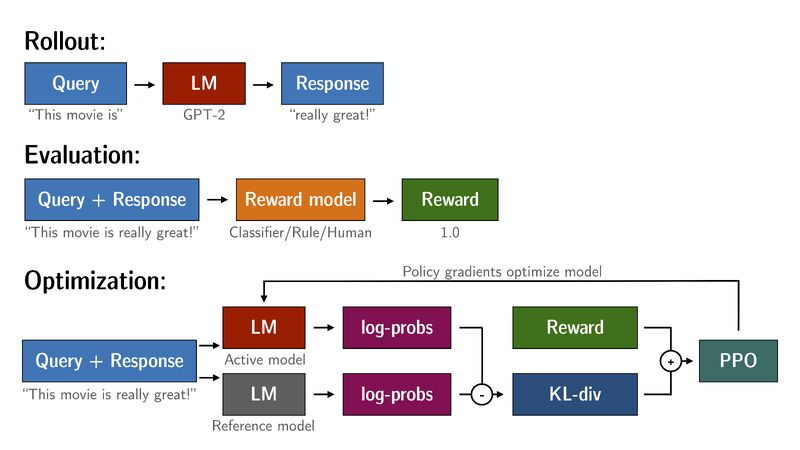
\includegraphics[width=\linewidth,keepaspectratio]{llm62}
\end{center}		


{\tiny (Ref: Linkedin Post on 11 Aug 2023 by -Katharina Koerner )}

\end{frame}
